\chapter{Identity Mixer\label{chp:idemix}}
\index{Identity Mixer|(}

Identity Mixer~\cite{CamenischLysyanskaya2001,IdemixCrypto2012} is an
attribute-based credential system, developed at IBM Research in Z\"urich, that
enables strong authentication\index{authentication} and privacy at the same time. The first
prototype~\cite{CamenischH02} was developed in 2002 and has been improved over
the years~\cite{BrickellCC2004,CamenischGroth2004}. An open source Java
implementation\footnote{\url{http://prime.inf.tu-dresden.de/idemix/}} was
released in 2010 as part of IBM's open innovation
initiative\footnote{\url{http://www.zurich.ibm.com/news/10/innovation.html}}.

The core of the Identity Mixer technology is the Camenisch-Lysyanskaya signature
scheme~\cite{CamenischLysyanskaya2003,Lysyanskaya2002}. This scheme is an ideal
building block for privacy-preserving technologies as Camenisch and Lysyanskaya
provide protocols for
\begin{enumerate}
  \item issuing signatures on committed values (such that the signer has no
    information about the signed value), that is, blind
    signatures~\cite{Chaum1983}, and
  \item proving knowledge of a signature on a committed value.
\end{enumerate}
Furthermore this scheme supports multiple messages to be signed at once. This
allows a number of attributes to be combined into a single credential. In
contrast to the U-Prove technology, an Identity Mixer credential can be
randomised (like the self-blindable credentials) allowing it to be used multiple
times while remaining anonymous.

In this chapter we focus on the core features of the Identity Mixer system:
credential issuance and selective disclosure of attributes. The technology
offers many more features that might be interesting to users of an
attribute-based credential system, but we focus on what can be achieved on a
smart card\index{smart card} with an acceptable performance~\cite{VullersAlpar2013}. Additional
options can still be added, but at the cost of an increased transaction time.

\section{Camenisch-Lysyanskaya Signature Scheme\label{sec:CL-scheme}}
\index{Camenisch-Lysyanskaya!signature scheme|(}

This description of the Camenisch-Lysyanskaya signature
scheme~\cite{CamenischLysyanskaya2003,Lysyanskaya2002} is based on the
direct anonymous attestation explanation by Camenisch~\cite{Camenisch2007} and
the specification of the Identity Mixer cryptographic
library~\cite{IdemixCrypto2012}. These documents include the efficiency
improvements which have been presented by Brickell, Camenisch, and
Chen~\cite{BrickellCC2004} and by Camenisch and Groth~\cite{CamenischGroth2004}.

\subsection{Keys}\label{sec:cl_keys}

The private key\index{Camenisch-Lysyanskaya!private key} in this scheme comprises two Sophie Germain primes $p'$ and $q'$.
The public key \index{Camenisch-Lysyanskaya!public key} consists of a special RSA modulus $n = p \cdot q$ where
$p = 2 \cdot p' + 1$ and $q = 2 \cdot q' + 1$ are safe primes. Furthermore we
need the following parameters from
$QR_n = \{ x \in \Z_n: y \in Z_n \land x = y^2 \mod n \}$, the group of
quadratic residues modulo $n$:
\begin{itemize}
  \item a generator $S \in QR_n$, with order $p' \cdot q'$, that generates
    $\langle S \rangle$, the subgroup of $QR_n$ in which all computations take
    place;
  \item a base $R_i = S^{x_i} \mod n$, where $x_i \in_R [2, p' \cdot q' - 1]$,
    for each message $m_i$ to be signed using this key; and
  \item an auxiliary value $Z = S^{x_z} \mod n$, where
    $x_z \in_R [2, p' \cdot q' - 1]$, such that all computations remain within
    $\langle S \rangle$.
\end{itemize}
Hence the resulting public key is $(n, S, Z, \{R_i\}_{i \in \M})$ where $\M$
denotes the set of message indices supported by this key.

\index{Camenisch-Lysyanskaya!public key!proof|(}
In order to guarantee that such a public key has been constructed correctly,
that is, all values are elements of $\langle S \rangle$, a proof of
correctness can be constructed (Algorithm~\ref{alg:CL-prove-key}, based
on~\cite[Appendix A]{BrickellCC2004}):
\begin{multline*}
  SPK \{ (\alpha_z, (\alpha_i)_{i \in \M}) : Z = S^{\alpha_z} \mod n
    \:\land\: \\ \forall_{i \in \M} R_i = S^{\alpha_i} \mod n
  \}(n, S, Z, \{R_i\}_{i \in \M})
\end{multline*}

\begin{algorithm}
  \caption{Proof correctness of a Camenisch-Lysyanskaya public key.}
  \label{alg:CL-prove-key}
  \addtolength{\baselineskip}{1mm}
  \begin{algorithmic}[1]
    \Function{CL-prove-key}{$(n, S, Z, \{R_i\}_{i \in \M})$}
      \ForAll{$j \in \H$}
        \State $u_j \gets \Call{Random}{~}$
        \State $Z'_j = S^{u_j} \mod n$
        \ForAll{$i \in \M$}
          \State $v_{(i,j)} \gets \Call{Random}{~}$
          \State $R'_{(i,j)} = S^{v_{(i,j)}} \mod n$
        \EndFor
      \EndFor

      \State $c \gets \Call{Hash}{n, S, Z, \{R_i\}_{i \in \M}, (Z'_j)_{j \in \H}, \{R'_{(i, j)}\}_{i \in \M, j \in \H}}$

      \ForAll{$j \in \H$}
        \State $r_j = u_j - c_j \cdot x_z \mod (p' \cdot q')$
        \ForAll{$i \in \M$}
          \State $s_{(i,\, j)} \gets v_{(i,\, j)} - c_j \cdot x_i \mod (p' \cdot q')$
        \EndFor
      \EndFor

      \Return $(c, \{r_j\}_{j \in \H}, \{s_{(i, j)}\}_{i \in \M,\, j \in \H})$
    \EndFunction
  \end{algorithmic}
\end{algorithm}

This proof uses binary challenges, hence we need to generate commitments and
responses for all bits of the challenge $\{c_j\}_{j \in \H}$, where $\H$
denotes the set of bits generated by the \textsc{Hash} function. These binary
challenges are necessary to satisfy the special soundness property of the
security proof~\cite[Section~3.5]{Camenisch2007}. Normally, one could just use
the challenge $c$ in combination with the strong RSA assumption to satisfy this
property, but in this case the strong RSA assumption does not hold since the
party that generated the key knows the factorisation of $n$.

% Special soundness: take two runs with the same commitment, but different
% challenges (and responses): (a, c, r) and (a, c', r').
%
% This gives y = g^{(r-r')/(c-c')}, hence witness w = (r-r')/(c-c').
% This can only be computed if:
% 1) c, c' are binary, thus delta(c) = +/- 1, or
% 2) under SRSA: delta(c) | delta(r) allows integer division
%       not(delta(c) | delta(r)) breaks SRSA, that is, it gives a root of g:
%            y^delta(c) = g^delta(r)    1 = a.delta(r) + b.delta(c)
%            g = g^{a.delta(r)} g^{b.delta(c)}
%              = y^{a.delta(c)} g^{b.delta(c)}
%              = (g^b y^a)^delta(c)
%
% The issuer knows the factorisation of n, and hence the order of the group, so
% SRSA does not hold in this case, so binary challenges is the only option here.

The proof can be verified using Algorithm~\ref{alg:CL-verify-key}, which
reconstructs the input of the hash based on the proof values and then checks
whether the output of the hash matches the given value. These values can be
reconstructed because:
\begin{equation*}
  Z^{c_j} \cdot S^{r_j}
  = (S^{x_z})^{c_j} \cdot S^{r_j}
  = (S^{x_z})^{c_j} \cdot S^{u_j - c_j x_z}
  = S^{u_j}
  = Z'_j \mod n \text{, and}
\end{equation*}
\begin{equation*}
  R_i^{c_j} \cdot S^{s_{(i,j)}}
  = (S^{x_i})^{c_j} \cdot S^{s_{(i,\, j)}}
  = (S^{x_i})^{c_j} \cdot S^{v_{(i,\, j)}-c_j x_i}
  = S^{v_{(i,j)}}
  = R'_{(i,j)} \mod n \text{.}
\end{equation*}

\begin{algorithm}
  \caption{Verify correctness of a Camenisch-Lysyanskaya public key.}
  \label{alg:CL-verify-key}
  \addtolength{\baselineskip}{1mm}
  \begin{algorithmic}[1]
    \Function{CL-verify-key}{$(n, S, Z, \{R_i\}_{i \in \M}), (c, \{r_j\}_{j \in \H}, \{s_{(i, j)}\}_{i \in \M, j \in \H})$}
      \ForAll{$j \in \H$}
        \State $Z'_j \gets Z^{c_j} \cdot S^{r_j} \mod n$
        \ForAll{$i \in \M$}
          \State $R'_{(i,j)} \gets R_i^{c_j} \cdot S^{r_{(i,\, j)}} \mod n$
        \EndFor
      \EndFor

      \If{$c \neq \Call{Hash}{n, S, Z, \{R_i\}_{i \in \M}, Z'_{j \in \H}, \{R'_{(i, j)}\}_{i \in \M,  j \in \H}}$}
        \Return \Call{Invalid}{}
      \EndIf

      \Return \Call{Valid}{}
    \EndFunction
  \end{algorithmic}
\end{algorithm}
\index{Camenisch-Lysyanskaya!public key!proof|)}

\subsection{Basic Signature Scheme}\label{sec:cl_basic}
\index{Camenisch-Lysyanskaya!signature|(}
In order to sign a collection of messages $\{m_i\}_{i \in \M}$, these $m_i$
first have to be aggregated into a single group element $Q$ according
to the following equation:\index{Camenisch-Lysyanskaya!message aggregation}
\begin{equation}\label{eqn:CL-aggregate}
  Q = \dfrac{Z}{S^v \cdot \prod_{i \in \M} R_i^{m_i}} \mod n\text,
\end{equation}
where $v$ is a random number. This value $v$ is used in
Section~\ref{sec:cl_blind} for blinding the messages that have to remain hidden,
and in Section~\ref{sec:cl_proof} to randomise the signature.

The actual signature generation process is similar to the RSA signature scheme.\index{Camenisch-Lysyanskaya!signature!generation}
The first step is the generation of a random prime $e$ which is used as the
ephemeral RSA public key for this signature. Next, the RSA private key
$d = e^{-1} \mod (p' \cdot q')$ corresponding to the public key $e$ is
computed. Finally, $A = Q^d \mod n$ is the RSA signature over the aggregated
messages. As a result the Camenisch-Lysyanskaya signature over the messages
$\{m_i\}_{i \in \M}$ is the triple $(A, e, v)$ (see
Algorithm~\ref{alg:CL-sign}).

\clearpage

\begin{algorithm}
  \caption{Generate a basic Camenisch-Lysyanskaya signature.}
  \label{alg:CL-sign}
  \addtolength{\baselineskip}{1mm}
  \begin{algorithmic}[1]
    \Function{CL-sign}{$\{m_i\}_{i \in \M}, (n, S, Z, \{R_i\}_{i \in \M}), (p', q')$}
      \State $v \gets \Call{Random}{~}$
      \State $U \gets S^v \mod n$
      \ForAll{$i \in \M$}
        \State $U \gets U \cdot R_i^{m_i} \mod n$
      \EndFor
      \State $Q \gets Z \cdot U^{-1} \mod n$

      \State $e \gets \Call{RandomPrime}{~}$
      \State $d \gets e^{-1} \mod (p' \cdot q')$
      \State $A \gets Q^d \mod n$

      \Return $(A, e, v)$
    \EndFunction
  \end{algorithmic}
\end{algorithm}

In order to verify such a Camenisch-Lysyanskaya signature $(A, e, v)$ the RSA
signature over the aggregated messages has to be verified. That is, the verifier
has to check the following equation:\index{Camenisch-Lysyanskaya!signature!verification}
\begin{equation}\label{eqn:CL-verify}
  A^e = \dfrac{Z}{S^v \cdot \prod_{i \in \M} R_i^{m_i}} \mod n
\end{equation}
This is equivalent to checking the following equation, as used in
Algorithm~\ref{alg:CL-verify}, such that it is not necessary to compute the
inverse:
\begin{equation}\label{eqn:CL-verify-Z}
  Z = A^e \cdot S^v \cdot \textstyle\prod_{i \in \M} R_i^{m_i} \mod n
\end{equation}

\begin{algorithm}
  \caption{Verify a basic Camenisch-Lysyanskaya signature.}
  \label{alg:CL-verify}
  \addtolength{\baselineskip}{1mm}
  \begin{algorithmic}[1]
    \Function{CL-verify}{$\{m_i\}_{i \in \M}, (A, e, v), (n, S, Z, \{R_i\}_{i \in \M})$}
      \State $Z' \gets A^e \cdot S^v \mod n$
      \ForAll{$i \in \M$}
        \State $Z' \gets Z' \cdot R_i^{m_i} \mod n$
      \EndFor

      \If{$Z \neq Z'$}
        \Return \Call{Invalid}{}
      \EndIf

      \Return \Call{Valid}{}
    \EndFunction
  \end{algorithmic}
\end{algorithm}
\index{Camenisch-Lysyanskaya!signature|)}

\subsection{Blind Signatures\label{sec:cl_blind}}
\index{Camenisch-Lysyanskaya!blind signature|(}
\begin{figure}[ht]
  \centering
  \includegraphics[scale=.45]{mscs/cl_blind-sign_simple}
  \caption{Protocol for generating blind signatures.}
  \label{msc:cl_blind-sign}
\end{figure}

Figure~\ref{msc:cl_blind-sign} depicts the protocol for generating blind
Camenisch-Lysyanskaya signatures. This protocol hides\index{hiding} the messages
$\{m_i\}_{i \in \M_H}$, where $\M_H \subseteq \M$, from the signer by generating a
commitment to these values and blinding them according to
Algorithm~\ref{alg:CL-blind-commit}. During this commitment phase these
messages are aggregated into a single element $U$ and hidden by the blinding
value $v'$. Note that the remaining messages $\{m_i\}_{i \in \M \setminus \M_H}$,
that are not hidden during this phase, are known by the signer.\index{Camenisch-Lysyanskaya!message aggregation}

\begin{algorithm}
  \caption{Prepare for a blind Camenisch-Lysyanskaya signature.}
  \label{alg:CL-blind-commit}
  \addtolength{\baselineskip}{1mm}
  \begin{algorithmic}[1]
    \Function{CL-blind-commit}{$\{m_i\}_{i \in \M_H}, (n, S, Z, \{R_i\}_{i \in \M})$}
      \State $v' \gets \Call{Random}{~}$

      \State $U \gets S^{v'} \mod n$
      \ForAll{$i \in \M_H$}
        \State $U \gets U \cdot R_i^{m_i} \mod n$
      \EndFor

      \Return $(U, v')$
    \EndFunction
  \end{algorithmic}
\end{algorithm}

In order to prove to the signer that the user actually knows the hidden
messages, the following proof of knowledge has to be carried out.
\begin{equation*}
  PK\{(\nu, \{\mu_i\}_{i \in \M_H}) :
    U = S^{\nu} \cdot \textstyle\prod_{i \in \M_H} R_i^{\mu_i} \mod n\}
\end{equation*}
This proof not only proves that the user knows the hidden messages, but also
that the value $U$ has been constructed correctly by the user. This can be
implemented as an interactive zero-knowledge protocol or using
Algorithms~\ref{alg:CL-prove-U} and~\ref{alg:CL-verify-U} which, respectively,
construct and verify a non-interactive proof of knowledge. The freshness of this
proof is guaranteed by a nonce $n_U$ provided by the signer. The verification
succeeds if the signer can successfully reconstruct the commitment $\tilde{U}$
on $U$. This reconstruction works because of the following equation.
\begin{align*}
  \hat{U}
  & = S^{\hat{v}'} \cdot U^{-c} \cdot
    \textstyle \prod_{i \in \M_H} R_i^{\hat{m}_i}
    = S^{\tilde{v}' + c \cdot v'} \cdot U^{-c} \cdot
    \textstyle\prod_{i \in \M_H} R_i^{\tilde{m}_i + c \cdot m_i} \\
  & = S^{\tilde{v}'} \cdot S^{c \cdot v'} \cdot U^{-c}
    \cdot \textstyle\prod_{i \in \M_H} R_i^{\tilde{m}_i}
    \cdot \textstyle\prod_{i \in \M_H} R_i^{c \cdot m_i} \\
  & = S^{\tilde{v}'} \cdot U^{-c} \cdot U^c
    \cdot \textstyle\prod_{i \in \M_H} R_i^{\tilde{m}_i}
    = S^{\tilde{v}'} \cdot \textstyle\prod_{i \in \M_H} R_i^{\tilde{m}_i} \\
  & = \tilde{U} \mod n
\end{align*}

\begin{algorithm}[t]
  \caption{Generate a proof of correctness for $U$.}
  \label{alg:CL-prove-U}
  \addtolength{\baselineskip}{1mm}
  \begin{algorithmic}[1]
    \Function{CL-prove-U}{$(U, v'), n_U, \{m_i\}_{i \in \M_H}, (n, S, Z, \{R_i\}_{i \in \M}))$}
      \State $\tilde{v}' \gets \Call{Random}{~}$
      \State $\tilde{U} \gets S^{\tilde{v}'} \mod n$
      \ForAll{$i \in \M_H$}
        \State $\tilde{m}_i \gets \Call{Random}{~}$
        \State $\tilde{U} \gets \tilde{U} \cdot R_i^{\tilde{m}_i} \mod n$
      \EndFor
      \State $c \gets \Call{Hash}{U, \tilde{U}, n_U}$
      \State $\hat{v}' \gets \tilde{v}' + c \cdot v'$
      \ForAll{$i \in \M_H$}
        \State $\hat{m}_i \gets \tilde{m}_i + c \cdot m_i$
      \EndFor

      \Return $(c, \hat{v}', \hat{m}_{i \in \M_H})$
    \EndFunction
  \end{algorithmic}
\end{algorithm}

\begin{algorithm}[t]
  \caption{Verify the proof of correctness for $U$.}
  \label{alg:CL-verify-U}
  \addtolength{\baselineskip}{1mm}
  \begin{algorithmic}[1]

    \Function{CL-verify-U}{$U, (c, \hat{v}', \hat{m}_{i \in \M_H}), n_U, (n, S, Z, \{R_i\}_{i \in \M})$}
      \State $\hat{U} \gets U^{-c} \cdot S^{\hat{v}'} \mod n$
      \ForAll{$i \in \M_H$}
        \State $\hat{U} \gets \hat{U} \cdot R_i^{\hat{m}_i} \mod n$
      \EndFor
      \If{$c \neq \Call{Hash}{U, \hat{U}, n_U}$}
        \Return \Call{Invalid}{}
      \EndIf

      \Return \Call{Valid}{}
    \EndFunction
  \end{algorithmic}
\end{algorithm}

The next step is the actual signing process. In this step the hidden messages,
aggregated in $U$, are combined with the remaining known messages
$\{m_i\}_{i \in \M \setminus \M_H}$ that will be included in the signature.
This process is very similar to the basic signature operation as given in
Algorithm~\ref{alg:CL-sign}. The main difference in
Algorithm~\ref{alg:CL-blind-sign} is the inclusion of the value $U$ received
from the user in the previous message aggregation step.

\begin{algorithm}
  \caption{Generate a blind Camenisch-Lysyanskaya signature.}
  \label{alg:CL-blind-sign}
  \addtolength{\baselineskip}{1mm}
  \begin{algorithmic}[1]

    \Function{CL-blind-sign}{$U, \{m_i\}_{i \in \M \setminus \M_H}, (n, S, Z, \{R_i\}_{i \in \M}), (p', q')$}
      \State $v'' \gets \Call{Random}{~}$
      \State $U \gets U \cdot S^{v''} \mod n$
      \ForAll{$i \in \M \setminus \M_H$}
        \State $U \gets U \cdot R_i^{m_i} \mod n$
      \EndFor
      \State $Q \gets Z \cdot U^{-1} \mod n$

      \State $e \gets \Call{RandomPrime}{~}$
      \State $d \gets e^{-1} \mod (p' \cdot q')$
      \State $A \gets Q^d \mod n$

      \Return $(A, e, v'')$
    \EndFunction
  \end{algorithmic}
\end{algorithm}

Furthermore, the signer provides the following proof of knowledge to show the
user that the signature has been constructed correctly.
\begin{equation*}
  PK\{(\delta) : A = \left(\dfrac{Z}{U \cdot S^{v''} \cdot
    \prod_{i \in \M \setminus \M_H} R_i^{m_i}} \right)^{\delta} \mod n \}
\end{equation*}
Again, this proof of knowledge can be implemented as an interactive
zero-knowledge protocol or as a non-interactive proof of knowledge.
Algorithms~\ref{alg:CL-prove-A} and~\ref{alg:CL-verify-A}, respectively,
construct and verify such a non-interactive proof with a nonce $n_A$ provided by
the user to guarantee the freshness. The commitment $\tilde{A}$ can be
reconstructed to verify the proof according to the following
equation\footnote{Note that in version~2.3.3 of the specification of the
Identity Mixer cryptographic library~\cite{IdemixCrypto2011}, the reconstructed
value $\hat{A}$ is incorrect, after reporting this to the authors it has been
corrected in version~2.3.4~\cite{IdemixCrypto2012}.}.
\begin{equation*}
  \hat{A}
   = A^{c + \hat{d} \cdot e}
   = Q^{e^{-1} \cdot (c + \hat{d} \cdot e)}
   = Q^{c \cdot e^{-1} + \hat{d}}
   = Q^{c \cdot e^{-1} + \tilde{d} - c \cdot e^{-1}}
   = Q^{\tilde{d}}
   = \tilde{A} \mod n
\end{equation*}

\begin{algorithm}
  \caption{Generate a proof of correctness for $A$.}
  \label{alg:CL-prove-A}
  \addtolength{\baselineskip}{1mm}
  \begin{algorithmic}[1]
    \Function{CL-prove-A}{$(A, e, v''), d, n_A, (n, S, Z, \{R_i\}_{i \in \M}), (p', q')$}
      \State $\tilde{d} \gets \Call{Random}{~}$
      \State $\tilde{A} \gets Q^{\tilde{d}} \mod n$

      \State $c \gets \Call{Hash}{Q, A, \tilde{A}, n_A}$

      \State $\hat{d} \gets \tilde{d} - c \cdot d \mod (p' \cdot q')$

      \Return $(c, \hat{d})$
    \EndFunction
  \end{algorithmic}
\end{algorithm}

\begin{algorithm}
  \caption{Verify the proof of correctness for $A$.}
  \label{alg:CL-verify-A}
  \addtolength{\baselineskip}{1mm}
  \begin{algorithmic}[1]
    \Function{CL-verify-A}{$(A, e, v''), (c, \hat{d}), n_A, (n, S, Z, \{R_i\}_{i \in \M})$}
      \State $Q \gets A^e \mod n$
      \State $\hat{A} \gets A^{c + \hat{d} \cdot e} \mod n$

      \If{$c \neq \Call{Hash}{Q, A, \hat{A}, n_A}$}
        \Return \Call{Invalid}{}
      \EndIf

      \Return \Call{Valid}{}
    \EndFunction
  \end{algorithmic}
\end{algorithm}

\begin{algorithm}
  \caption{Finish a blind Camenisch-Lysyanskaya signature.}
  \label{alg:CL-blind-finish}
  \addtolength{\baselineskip}{1mm}
  \begin{algorithmic}[1]
    \Function{CL-blind-finish}{$v', (A, e, v'')$}
      \State $v \gets v' + v''$

      \Return $(A, e, v)$
    \EndFunction
  \end{algorithmic}
\end{algorithm}

Finally, the user has to complete the signature according to
Algorithm~\ref{alg:CL-blind-finish} which combines the blinding values of the
user and signer, $v'$ and $v''$ respectively, to become the randomisation
value $v$ of the Camenisch-Lysyanskaya signature $(A, e, v)$. This signature can
now be verified using the verification procedure from the basic signature scheme
(Algorithm~\ref{alg:CL-verify}) or it can be used to prove knowledge of this
signature as described in the following section.

\index{Camenisch-Lysyanskaya!blind signature|)}

\subsection{Proving Knowledge of a Signature\label{sec:cl_proof}}
\index{Camenisch-Lysyanskaya!signature!proving knowledge|(}
Blind signatures hide\index{hiding} (a number of) the messages from the signer during
signature generation. The goal of proving knowledge of a signature is to hide
(a number of) the messages from the verifier during signature verification as
well as to hide the actual value of the signature to prevent traceability. This
process, as depicted in Figure~\ref{msc:cl_prove-sign}, allows the user to prove
that she has a signature over one or more (possibly hidden) messages without
revealing the actual signature to the verifier.

\begin{figure}[b]
  \centering
  \includegraphics[scale=.45]{mscs/cl_prove-sign_simple}
  \caption{Protocol for proving knowledge of a signature.}
  \label{msc:cl_prove-sign}
\end{figure}

To hide the Camenisch-Lysyanskaya signature $(A, e, v)$ and prevent linkability
based on the signature values $A$, $e$, and $v$ the signature is randomised,
using Algorithm~\ref{alg:CL-randomise}. First a randomisation value $r$ is
generated to randomise the RSA signature value $A$. Next the value $v$ is
adjusted such that the signature remains valid, that is, it still satisfies
(\ref{eqn:CL-verify}):
\begin{align*}
  A'^e
  & = (A \cdot S^r)^e
  = A^e \cdot S^{e \cdot r} \\
  &= \dfrac{S^{e \cdot r} \cdot Z}{S^v \cdot \prod_{i \in \M} R_i^{m_i}}
  = \dfrac{S^{- e \cdot r} \cdot S^{e \cdot r} \cdot Z}{S^{- e \cdot r} \cdot S^v \cdot \prod_{i \in \M} R_i^{m_i}} \\
  &= \dfrac{Z}{S^{v - e \cdot r} \cdot \prod_{i \in \M} R_i^{m_i}}
  = \dfrac{Z}{S^{v'} \cdot \prod_{i \in \M} R_i^{m_i}} \mod n
\end{align*}

\begin{algorithm}
  \caption{Randomise a Camenisch-Lysyanskaya signature.}
  \label{alg:CL-randomise}
  \addtolength{\baselineskip}{1mm}
  \begin{algorithmic}[1]
    \Function{CL-randomise}{$(A, e, v), (n, S, Z, \{R_i\}_{i \in \M})$}
      \State $r \gets \Call{Random}{~}$
      \State $A' \gets A \cdot S^r \mod n$
      \State $v' \gets v - e \cdot r$

      \Return $(A', e, v')$
    \EndFunction
  \end{algorithmic}
\end{algorithm}

This randomisation operation only effectively randomises the $A$ value of the
signature. Hence it is required to hide the $e$ and $v'$ values using a
zero-knowledge proof when revealing this randomised signature and the messages
$\{m_i\}_{i \in \M_D}$ disclosed to the verifier. Furthermore the following proof hides\index{hiding} the messages
$\{m_i\}_{i \in \M \setminus \M_D}$ that the user does not wish to disclose to the
verifier.
\begin{equation*}
  PK\{(\epsilon, \nu, \{\mu_i\}_{i \in \M \setminus \M_D}) :
    Z = A'^{\epsilon} \cdot S^{\nu}
    \cdot \textstyle\prod_{i \in \M \setminus \M_D} R_i^{\mu_i}
    \cdot \textstyle\prod_{i \in \M_D} R_i^{m_i} \mod n \}
\end{equation*}

Algorithm~\ref{alg:CL-prove-D} describes the operations that have to be
performed to generate a proof of knowledge of a signature and the hidden
messages. This proof can then be verified to check the correctness of the
signature over the disclosed messages using Algorithm~\ref{alg:CL-verify-D}.
Note that the messages $\{m_i\}_{i \in \M_D}$ disclosed by the user are known
by the verifier and are input to the verification algorithm. Similar to the
previous proofs in this scheme the verification relies on the reconstruction of
the commitments, which in this case is possible because of the following
equation.

\begin{algorithm}
  \caption{Prove knowledge of a Camenisch-Lysyanskaya signature.}
  \label{alg:CL-prove-D}
  \addtolength{\baselineskip}{1mm}
  \begin{algorithmic}[1]
    \Function{CL-prove-D}{$\{m_i\}_{i \in \M \setminus \M_D}, (A', e, v'), n_D, (n, S, Z, \{R_i\}_{i \in \M})$}
      \State $\tilde{e} \gets \Call{Random}{~}$
      \State $\tilde{v} \gets \Call{Random}{~}$
      \State $\tilde{Z} \gets {A'}^{\tilde{e}} \cdot S^{\tilde{v}} \mod n$

      \ForAll{$i \in \M \setminus \M_D$}
        \State $\tilde{m}_i \gets \Call{Random}{~}$
        \State $\tilde{Z} \gets \tilde{Z} \cdot R_i^{\tilde{m}_i} \mod n$
      \EndFor

      \State $c \gets \Call{Hash}{A', \tilde{Z}, n_D}$

      \State $\hat{e} \gets \tilde{e} + c \cdot e$
      \State $\hat{v} \gets \tilde{v} + c \cdot v'$
      \ForAll{$i \in \M \setminus \M_D$}
        \State $\hat{m}_i \gets \tilde{m}_i + c \cdot m_i$
      \EndFor

      \Return $(c, A', \hat{e}, \hat{v}, \{\hat{m}_i\}_{i \in \M \setminus \M_D})$
    \EndFunction
  \end{algorithmic}
\end{algorithm}

\begin{align*}
  \hat{Z}
  & = Z^{-c} \cdot A'^{\hat{e}} \cdot S^{\hat{v}}
    \cdot (\textstyle\prod_{i \in \M_D} R_i^{m_i})^c
    \cdot \textstyle\prod_{i \in \M \setminus \M_D} R_i^{\hat{m}_i} \\
  & = Z^{-c} \cdot A'^{\tilde{e} + c \cdot e} \cdot S^{\tilde{v} + c \cdot v'}
    \cdot \textstyle\prod_{i \in \M_D} R_i^{c \cdot m_i}
    \cdot \textstyle\prod_{i \in \M \setminus \M_D} R_i^{\tilde{m}_i + c \cdot m_i} \\
  & = Z^{-c} \cdot A'^{\tilde{e}} \cdot A'^{c \cdot e}
    \cdot S^{\tilde{v}'} \cdot S^{c \cdot v'}
    \cdot \textstyle\prod_{i \in \M_D} R_i^{c \cdot m_i}
    \cdot \textstyle\prod_{i \in \M \setminus \M_D} R_i^{\tilde{m}_i}
    \cdot \textstyle\prod_{i \in \M \setminus \M_D} R_i^{c \cdot m_i} \\
  & = Z^{-c}
    \cdot (A'^{e} \cdot S^{v'} \cdot \textstyle\prod_{i \in \M} R_i^{m_i})^c
    \cdot A'^{\tilde{e}} \cdot S^{\tilde{v}'}
    \cdot \textstyle\prod_{i \in \M \setminus \M_D} R_i^{\tilde{m}_i} \\
  & = (A'^{e} \cdot S^{v'} \cdot \textstyle\prod_{i \in \M} R_i^{m_i})^{-c}
    \cdot (A'^{e} \cdot S^{v'} \cdot \textstyle\prod_{i \in \M} R_i^{m_i})^c
    \cdot A'^{\tilde{e}} \cdot S^{\tilde{v}'}
    \cdot \textstyle\prod_{i \in \M \setminus \M_D} R_i^{\tilde{m}_i} \\
  & = A'^{\tilde{e}} \cdot S^{\tilde{v}'}
    \cdot \textstyle\prod_{i \in \M \setminus \M_D} R_i^{\tilde{m}_i} \\
  & = \tilde{Z} \mod n
\end{align*}
Note that this equation uses (\ref{eqn:CL-verify-Z}) and hence depends on the
validity of the signature used to generate this proof. If the triple $(A, e, v)$
is not a valid signature, that is (\ref{eqn:CL-verify-Z}) does not hold, the
proof will fail.

\begin{algorithm}[t]
  \caption{Verify the signature proof of knowledge.}
  \label{alg:CL-verify-D}
  \addtolength{\baselineskip}{1.5mm}

  \begin{algorithmic}[1]
    \Function{CL-verify-D}{$(c, A', \hat{e}, \hat{v}, \{\hat{m}_i\}_{i \in \M \setminus \M_D}, \{m_i\}_{i \in \M_D}), n_D, (n, S, Z, \{R_i\}_{i \in \M})$}
      \State $\hat{Z} \gets Z^{-c} \cdot A'^{\hat{e}} \cdot S^{\hat{v}} \mod n$
      \ForAll{$i \in \M_D$}
        \State $\hat{Z} \gets \hat{Z} \cdot R_i^{c \cdot m_i} \mod n$
      \EndFor
      \ForAll{$i \in \M \setminus \M_D$}
        \State $\hat{Z} \gets \hat{Z} \cdot R_i^{\hat{m}_i} \mod n$
      \EndFor

      \If{$c \neq \Call{Hash}{A', \hat{Z}, n_D}$}
        \Return \Call{Invalid}{}
      \EndIf
      \Return \Call{Valid}{}
    \EndFunction
  \end{algorithmic}
\end{algorithm}
\index{Camenisch-Lysyanskaya!signature!proving knowledge|)}
\index{Camenisch-Lysyanskaya!signature scheme|)}

\section{Identity Mixer Credentials}
\index{Identity Mixer!credentials}

The Identity Mixer technology is tightly built upon the Camenisch-Lysyanskaya
signature scheme and its protocols. The blind signature scheme provides the
issuance protocol where the messages become the contents of the credential. The
protocol for proving knowledge of a signature is used as the credential
verification protocol.

\index{Identity Mixer!issuance}
\index{Identity Mixer!issuance|see{Camenisch-Lysyanskaya, blind signature}}
An Identity Mixer credential contains a master secret $s$, which belongs to the
user and is never revealed, and a collection of attributes
$\{a_i\}_{i \in \mathcal{A}}$, where $\mathcal{A}$ denotes the set of
attribute indices.\index{attribute!index set} Hence, the sets of message indices for the issuance protocol
become $\{m_i\}_{i \in \M_H} = \{s\}$ and $\M = \M_H \cup \mathcal{A}$. As a result of the
issuance protocol the user obtains a signature $(A, e, v)$ over these values
which completes the credential.

\clearpage
\begin{figure}[ht]
  \centering
  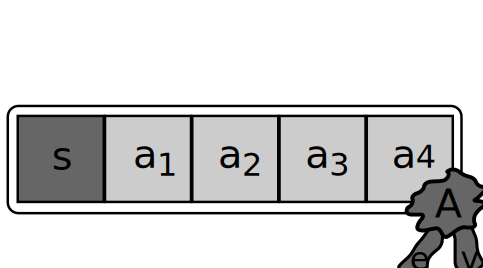
\includegraphics[scale=.45]{images/idemix-credential}
  \caption{A visual representation of an Identity Mixer credential.}
  \label{fig:idemix-credential}
\end{figure}

\noindent To summarise, an Identity Mixer credential, as depicted in
Figure~\ref{fig:idemix-credential}, consists of:
\begin{itemize}
  \item the user's master secret $s$,
  \item a collection of attributes $\{a_i\}_{i \in \mathcal{A}}$, and
  \item a signature $(A, e, v)$, over the user's master secret and the attributes, where
    $A = \left(\dfrac{Z}{S^v \cdot R_s^{s} \cdot \prod_{i \in \A} R_i^{a_i}}\right)^d \mod n$
    and $d = e^{-1} \mod (p' \cdot q')$.
\end{itemize}

\index{Identity Mixer!selective disclosure}
\index{Identity Mixer!selective disclosure|see{Camenisch-Lysyanskaya, signature, proving knowledge}}
This credential can now be used with the protocol for proving knowledge of a
signature to selectively disclose the attributes to a verifier. In this case the
set of disclosed messages $\M_D \subseteq \mathcal{A}$ is a selection of the
attributes contained in the credential. Using Algorithm~\ref{alg:CL-prove-D} the
user can now generate a proof of knowledge that can be sent to the verifier in
order to reveal the attributes and to prove that they are signed by the issuer.

This is the core of the Identity Mixer system that we have implemented on a
smart card,\index{smart card} for extensions of this proof which provide more features we refer
the reader to the specification of the Identity Mixer
technology~\cite{IdemixCrypto2012}.

\subsection{Direct Anonymous Attestation\label{sec:DAA}}
\index{direct anonymous attestation}
Direct anonymous attestation~\cite{BrickellCC04} is a technology based on
Identity Mixer, but it omits the attributes, hence $\M = \M_H$ and
$\M_D = \emptyset$. It allows a user to convince a verifier that she uses a
platform that has embedded a certified hardware module\footnote{Direct anonymous attestation has been adopted in 2004
by the Trusted Computing Group in the Trusted Platform Module specification as
the method for remote authentication\index{authentication!remote} of a hardware module.} by proving knowledge
of the signature that certifies the module. The protocol protects the user's
privacy: if she talks to the same verifier twice, the verifier is not able to
tell whether or not he communicates with the same user as before or with a
different one.

\section{Identity Mixer on Smart Cards}
\index{smart card}

We are not the first to develop an implementation of the Identity Mixer on a 
smart card. In 2009 Bichsel et al.~\cite{BichselCGS2009} implemented a minimal
Identity Mixer system on a Java Card\index{Java Card} whereas Sterckx et al.~\cite{Sterckx09}
did the same for direct anonymous attestation. They provide the first
implementations of this technology on smart cards. The major drawback of these
implementations is the running time of several seconds which is still too much
for being really practical.

\begin{figure}[ht]
  \centering
  \begin{subfigure}{0.45\textwidth}
    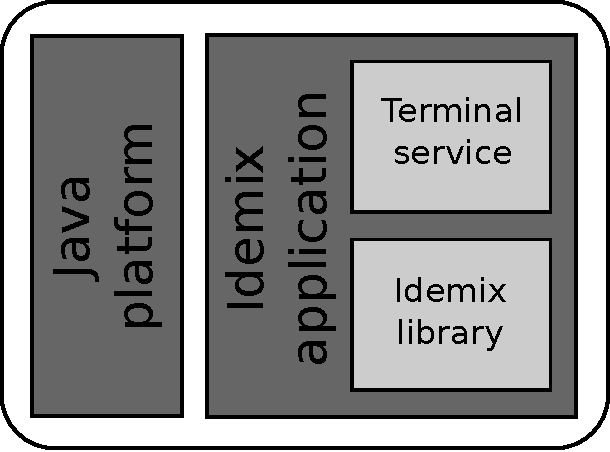
\includegraphics[scale=.45]{images/idemix-terminal-architecture}
    \caption{Terminal}
    \label{fig:terminal-architecture}
  \end{subfigure}
  \qquad
  \begin{subfigure}{0.45\textwidth}
    \includegraphics[scale=.45]{images/idemix-card-architecture}
    \caption{Card}
    \label{fig:card-architecture}
  \end{subfigure}
  \caption{System architecture for Identity Mixer on a smart card.}
  \label{fig:architecture}
\end{figure}

Our system consists of two parts, depicted in Figure~\ref{fig:architecture}, a
terminal~(\subref{fig:terminal-architecture}) which interacts with a
card~(\subref{fig:card-architecture}) using APDUs.\index{APDU} The terminal application is
written in Java and uses the Identity Mixer cryptographic library\footnote{The
library is available for download at \url{https://prime.inf.tu-dresden.de/idemix/}
while our patches can be found at \url{https://github.com/credentials/idemix_library}.}
provided by IBM Research. Thanks to Patrick Bichsel, version 2.3.4 of this
library provides interfaces for the various roles in the protocols such that we
could create an extension to this library, the terminal
service\footnote{\url{https://github.com/credentials/idemix_terminal}}, which
takes care of all smart card specifics. The service implements the user roles of
the Identity Mixer issuance and verification protocols, described by the
\texttt{Recipient} and \texttt{Prover} interfaces respectively. These
interfaces are implemented by translating all Java method calls from the
library into the corresponding APDU commands and converting the Java data types
to raw byte arrays, suitable for APDU communication.

The Identity Mixer application\footnote{\url{https://github.com/pimvullers/idemix_multos/}}
on the card takes care of handling the incoming APDUs\index{APDU} and storing the values
into the internal data structures. While handling the communication with the
terminal is the largest part of the application, the main part is the
implementation of the cryptographic operations for the Identity Mixer protocols.
This allows the card to perform the user roles without depending on the terminal
for any computations or proof generation. The only thing the terminal is
responsible for is providing the data in the correct format.

\subsection{Smart Card Implementation}

Just as with the U-Prove implementation, we have chosen to use the MULTOS\index{MULTOS} C
interface to do our prototype implementation of Identity Mixer. The programming
environment is convenient for smart card programming and allows us some more
flexibility for memory management. It will be explained below why this is
crucial.

Implementing the Identity Mixer specification did not turn out to be that hard
in the beginning, the available API makes it easy to implement the cryptographic
protocol. In principle, it is a direct translation from the mathematical
description to API calls. The only API restriction we came across was that the
\texttt{ModularExponentiation} function does not accept exponents larger than
the modulus size. In our case this only involves exponentiations with base $S$
(see details in Section~\ref{sec:CL-scheme}). Hence we added a function
\texttt{SpecialModularExponentiation} which implements the same method as used
by Bichsel et al.~\cite{BichselCGS2009}, that is, splitting one exponentiation
up into two\footnote{This method actually requires three exponentiations, but
we can precompute one exponentiation during initialisation, since we only need
this method for the base $S$.} exponentiations and one multiplication.

Our initial implementation only used static memory to store the variables. This
allowed us to work without thinking about which memory segment to use. The
drawback of this approach was a bad performance caused by the EEPROM\index{EEPROM} memory
which takes a long time, compared to RAM,\index{RAM} to write new values.

Once we had a functionally correct implementation, we started to optimise. This
was done by moving the buffer, which stores the intermediate results for larger
computations, to the public memory. The next step was to move the session
variables to the dynamic memory, which required careful organisation due to the
limited amount of available storage. However, when the dynamic memory use
increased the stack-based execution model started to cause trouble.

Initially, the stack could use the full size of the dynamic memory, such that
we had sufficient space to use functions and put the (relatively) large input
values on the stack. When using the C-interface, the compiler takes care of
managing the stack and putting input values on it when an instruction needs
this. However, this makes it difficult to get an idea on how much space the
stack actually needs. By trial and error, we discovered that we used quite some
amount of memory for the stack, which left us with only limited amount of space
for session variables.

To improve this situation, we reduced the number of function calls by inlining
some convenience functions. We also switched to using global variables instead
of function parameters, such that when we use a function, it does not require
much space on the stack. To get the last few, often used, variables into RAM,\index{RAM}
we decided to split up some computations into smaller parts such that the
values to be put on the stack also get smaller. For example, additions can be
computed using addition with carry, and multiplications using grade-school
multiplication. This adds a number of extra operations, but it is worth the
memory gain which results in improved performance.

Finally, we translated most parts of the cryptographic code to MEL assembly
which allowed us to optimise the use of stack and reduce the amount of memory
operations during calculations. This was required since the provided C-functions
moved the values from the stack to the variable locations, while they are needed
again in the next operation. By doing this we could reduce the amount of memory
required for intermediate values which in the end allowed us to get all
necessary variables in RAM.\index{RAM}

\section{Performance Results\label{sec:IM-performance}}

There are two important performance measures: the time it takes to issue a new
credential to the card, and the running time of the verification protocol.

For these performance tests we've used, where possible, the same test vectors as
with the U-Prove implementation in order to get comparable results (see
Chapter~\ref{chp:discussion} for a detailed comparison). Furthermore, our
implementation uses a modulus size of 1024~bits, which provides a minimal level
of security, but an acceptable performance. Given this size of the modulus, and
hence the size of all group elements, we can support at most 5 attributes per
credential in our implementation.

For issuance, we measured the running time of the protocol and determined how
much time was actually spent on computations and which part was used to transfer
and store the values (marked as overhead; see Figure~\ref{fig:issuance}). From
these results we can conclude that the number of attributes included in a
credential has only a minimal effect on the computations. An increase in the
number of attributes does, however, result in an increase of the overhead of
approximately 100 milliseconds per attribute.

\begin{figure}[t]
  \centering
  \includegraphics{images/idemix-issuance.mps}

  \caption[Identity Mixer credential issuance times for various numbers of attributes.]{
    Identity Mixer credential issuance times for various numbers of attributes
    (\raisebox{-.8\dp\strutbox}{\includegraphics{images/box-dark.mps}}:~computation time,
      \raisebox{-.8\dp\strutbox}{\includegraphics{images/box-light.mps}}:~overhead).}
  \label{fig:issuance}
\end{figure}

Sterckx et al.~\cite{Sterckx09} implement the direct anonymous attestation\index{direct anonymous attestation}
protocol, which is derived from the Identity Mixer protocols, on a Java~Card\index{Java Card}.
With a 1024~bits modulus they achieve a running time of 2.4~seconds of which
19\% is overhead, which gives a computation time of approximately 1.9~seconds.
This is good, and in line with the results we got, but unfortunately the direct
anonymous attestation\index{direct anonymous attestation} protocol does not support any attributes as it is just
targeted at anonymous authentication\index{authentication!anonymous} and hence only uses a secret key.

Bichsel et al.~\cite{BichselCGS2009} from IBM Research Z\"urch also implemented
a variant of the direct anonymous attestation\index{direct anonymous attestation} protocol on a Java~Card\index{Java Card}. They
report a running time of 7.4~seconds for a modulus size of 1280~bits, which is
larger than the 1024~bits we used. It is unclear, however, which transaction
time they measured. But again, this implementation does not include any
attributes.

For selective disclosure, we measured the running times of four configurations
(see Figure~\ref{fig:proving}). These configurations have been chosen because
two is the smallest number of attributes for which selective disclosure makes
sense and five is the largest number of attributes that we can currently keep in
memory while not using EEPROM\index{EEPROM} for computations during the transaction. By
comparing these graphs, it is clear that each attribute that is disclosed
reduces the computation time with roughly 100 milliseconds. Also, the scenario
in which all attributes results in similar computation times, with only slightly
increased overhead for the large number of attributes that have to be sent to
the terminal.

\begin{figure}[ht]
  \centering
  \begin{subfigure}[b]{0.45\textwidth}
    \includegraphics{images/idemix-2attr.mps}
    \caption{2 stored attributes}
    \label{fig:2attr-sle78}
  \end{subfigure}
  \begin{subfigure}[b]{0.45\textwidth}
    \includegraphics{images/idemix-4attr.mps}
    \caption{4 stored attributes}
    \label{fig:4attr-sle78}
  \end{subfigure}

  \vspace{5mm}

  \begin{subfigure}[b]{0.45\textwidth}
    \includegraphics{images/idemix-3attr.mps}
    \caption{3 stored attributes}
    \label{fig:3attr-sle78}
  \end{subfigure}
  \begin{subfigure}[b]{0.45\textwidth}
    \includegraphics{images/idemix-5attr.mps}
    \caption{5 stored attributes}
    \label{fig:5attr-sle78}
  \end{subfigure}

  \caption[Identity Mixer credential verification times for different configurations.]{
    Identity Mixer credential verification times for different configurations
    (\raisebox{-.8\dp\strutbox}{\includegraphics{images/box-dark.mps}}:~computation time,
      \raisebox{-.8\dp\strutbox}{\includegraphics{images/box-light.mps}}:~overhead).}
  \label{fig:proving}
\end{figure}

Comparing our work with the implementations by Sterckx et al.~\cite{Sterckx09}
and Bichsel et al.~\cite{BichselCGS2009} makes no real sense since they do not
offer selective disclosure of attributes. It is, however, clear that our
implementation provides a significant performance improvement over these
implementations. For example, Sterckx et al. need 4.2 seconds to hide only the
secret key while our implementation can hide the secret key and two attributes
of a single credential in 1.1 seconds.

\index{Identity Mixer|)}
